
Fig.~\ref{code:message} shows a second LM program, a message routing program
that simulates message transmission through a network of nodes.  Predicate
\code{edge/2} represents the connections between nodes, predicate
\code{message/3} contains the message content and the route list, and
predicate \code{processed/2} keeps count of the number of messages routed at
each node.

\begin{figure}[h!]
\begin{Verbatim}[numbers=left,commandchars=\*\{\},fontsize=\codesize]
type edge(node, node Neighbor).
type linear message(node, string Content, list node Routing).
type linear processed(node, int Total).

!edge(A, B),*label{line:language:message_first1}
message(A, Content, [B | L]),
processed(A, N)
   -o message(B, Content, L),
      processed(A, N + 1).*label{line:language:message_first2}

message(A, Content, []),*label{line:language:message_second1}
processed(A, N)
   -o processed(A, N + 1).*label{line:language:message_second2}

!edge(@1, @2). !edge(@2, @3). !edge(@3, @4). !edge(@1, @3).
processed(@1, 0). processed(@2, 0). processed(@3, 0). processed(@4, 0).
message(@1, "hello world", [@3, @4]).*label{line:language:message_message}
\end{Verbatim}
\caption{Code for routing messages in a graph. There is only one message ("hello
world") to route through nodes \code{@3} and \code{@4}.}
\label{code:message}
\end{figure}

The first rule
(lines~\ref{line:language:message_first1}-\ref{line:language:message_first2})
grabs the next node in the route list (third argument of \code{message/3}) and
ensures that a communication edge exists (through \code{edge(A,~B)}). We
increase the number of processed messages by consuming \code{processed(A,~N)}
and deriving \code{processed(A,~N+1)}.  When the route list is empty, the
message has reached its destination and thus it is consumed (rule in lines
\ref{line:language:message_first1}-\ref{line:language:message_first2}).  Note
that we only need to send one message since there is only one \code{message}
axiom (line~\ref{line:language:message_message}).

In Fig.~\ref{fig:message_trace} we present an execution trace of the message
routing program.  The database is represented as a graph structure where the
edges represent the \code{edge/2} initial facts. In
Fig.~\ref{fig:message_trace}~(a) the database is initialized with the program's
initial facts. Note that the initial \code{message/3} fact is instantiated at node
\code{@1}. After applying rule 1, we get the database represented in
Fig.~\ref{fig:message_trace}~(b), where the message has been derived at node
\code{@3}. After applying rule 1 again, the message is then routed to node
\code{@4} (Fig.~\ref{fig:message_trace}~(c)) where it will be consumed
(Fig.~\ref{fig:message_trace}~(d)).

\begin{figure}[h]
        \centering
        \begin{subfigure}[b]{0.4\textwidth}
                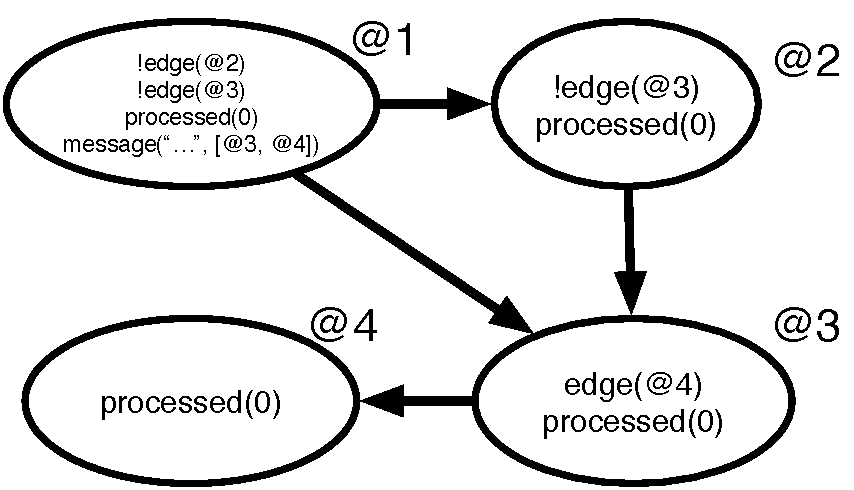
\includegraphics[width=\textwidth]{figures/message/message_trace1}
                \caption{Initial database.}
                \label{fig:message_trace1}
        \end{subfigure}%
        ~
        \begin{subfigure}[b]{0.4\textwidth}
                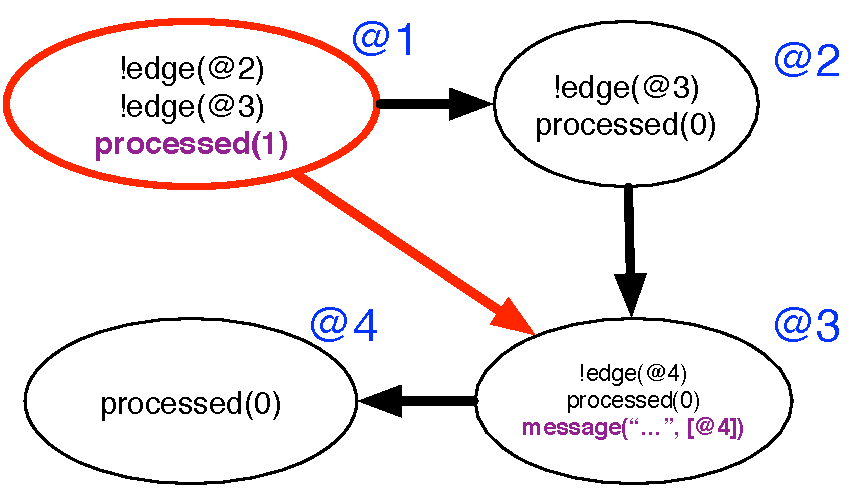
\includegraphics[width=\textwidth]{figures/message/message_trace2}
                \caption{After applying rule 1 at node \code{@1}.}
                \label{fig:message_trace2}
        \end{subfigure}\\
        \begin{subfigure}[b]{0.4\textwidth}
                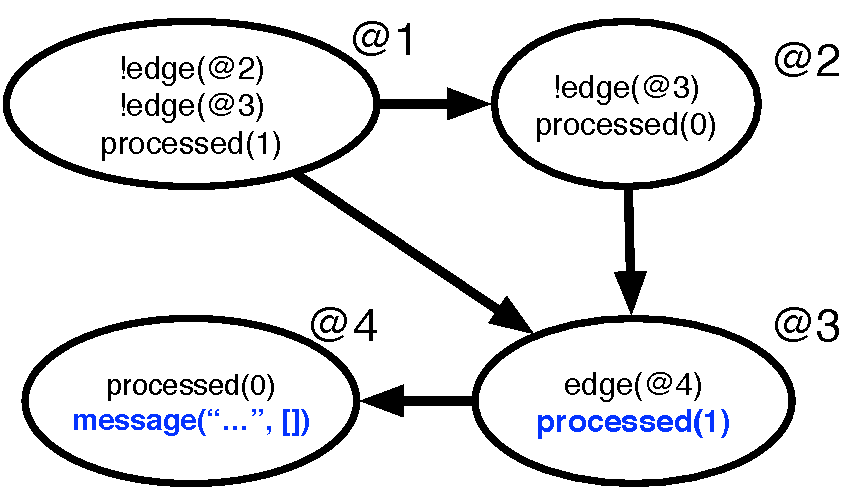
\includegraphics[width=\textwidth]{figures/message/message_trace3}
                \caption{After applying rule 1 at node \code{@3}.}
                \label{fig:message_trace3}
        \end{subfigure}%
        ~
        \begin{subfigure}[b]{0.4\textwidth}
                  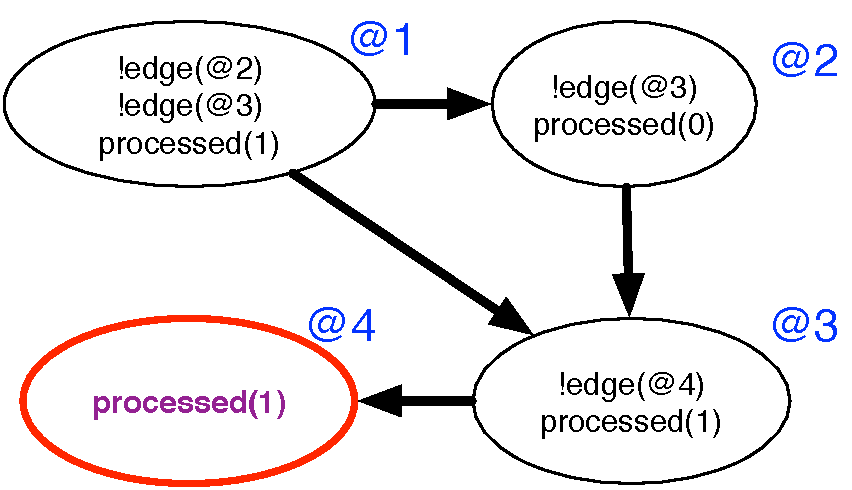
\includegraphics[width=\textwidth]{figures/message/message_trace4}
                  \caption{After applying rule 2 (nodes \code{@4}).}
                  \label{fig:message_trace4}
          \end{subfigure}
        \caption{An execution trace for the message program. The message "hello
        world" travels from node \code{@1} to node \code{@4}.}\label{fig:message_trace}
\end{figure}

